\documentclass{beamer}
\usepackage{graphicx}
\usepackage{hyperref}
\usepackage{tikz}
\usetikzlibrary{arrows.meta, positioning}
\usepackage{array}
\usepackage{amsmath}
\usepackage[svgnames]{xcolor}
\usepackage{listings}

\title{Introduction to Recommender Systems}
\author{Lecture Transcript}
\date{}

\begin{document}

% \frame{\titlepage}

\begin{frame}[plain]
    \begin{center}
        {\LARGE \textbf{Recommender Systems: Machine Learning Models for Customer Prediction}}
    \end{center}
\end{frame}

\begin{frame}{Overview of the Project}
\begin{itemize}
    \item Build a recommender system using explicit movie ratings provided by users.
    \item Recommender systems are a specialized type of machine learning model.
    \item Recommender systems predict items for users that they have never seen before or interacted with explicitly (e.g., by adding to favorites or making a purchase).
    \item Train the system on explicit user ratings.
    \item Test how accurately the algorithm can predict ratings for movies the users have already seen and rated.
\end{itemize}
\end{frame}

\begin{frame}[plain]
    \begin{center}
        {\LARGE \textbf{Introduction to Recommender Systems}}
    \end{center}
\end{frame}

\begin{frame}{What a Recommender System Is}
\begin{itemize}
    \item A specialized type of machine learning system.
    \item Predicts \textbf{ratings} or \textbf{preferences} a user might assign to an item.
    \item Recommends items based on:
    \begin{itemize}
        \item User's past behavior.
        \item Behavior of other users.
    \end{itemize}
    \item Often presented as \textbf{Top-N Recommendations}:
    \begin{itemize}
        \item A sorted list of items a user might like.
    \end{itemize}
\end{itemize}
\end{frame}

\begin{frame}{Examples of Recommender Systems}
\begin{itemize}
    \item Common names:
    \begin{itemize}
        \item Recommender engines
        \item Recommendation systems
        \item Recommendation platforms
    \end{itemize}
    \item Examples in practice:
    \begin{itemize}
        \item \textbf{Amazon}: Product recommendations based on user interactions and global customer data.
        \item \textbf{Netflix}: Movie recommendations based on user preferences and other users' preferences.
        \item \textbf{Music platforms}: Song recommendations.
        \item \textbf{Dating apps}: People recommendations.
    \end{itemize}
\end{itemize}
\end{frame}

\begin{frame}{Applications of Recommender Systems}
\begin{itemize}
    \item Recommender systems can suggest:
    \begin{itemize}
        \item Physical products.
        \item Digital content (e.g., music, videos).
        \item Services or experiences.
    \end{itemize}
    \item The key is learning user preferences over time and blending them with insights from others.
\end{itemize}
\end{frame}

\begin{frame}[plain]
    \begin{center}
        {\LARGE \textbf{Understanding You through Implicit and Explicit Ratings}}
    \end{center}
\end{frame}

% Slide: Introduction
\begin{frame}{How Do Recommender Systems Work?}
\begin{itemize}
    \item Recommender systems aim to understand you — and everyone else.
    \item They collect data about your preferences and compare them with others.
    \item The goal: recommend items you might like based on patterns and behaviors.
\end{itemize}
\end{frame}

% Slide: Data Sources
\begin{frame}{Sources of Data}
\begin{itemize}
    \item Recommender systems need data to understand user interests.
    \item Two main types:
    \begin{itemize}
        \item \textbf{Explicit Feedback}
        \item \textbf{Implicit Behavior}
    \end{itemize}
\end{itemize}
\end{frame}

% Slide: Explicit Feedback
\begin{frame}{Explicit Feedback}
\begin{itemize}
    \item Users rate items directly (e.g., 1–5 stars, thumbs up/down).
    \item Examples:
    \begin{itemize}
        \item Rating an online course.
        \item Giving a movie 4 out of 5 stars.
    \end{itemize}
    \item Benefits:
    \begin{itemize}
        \item Clear indication of preferences.
    \end{itemize}
    \item Limitations:
    \begin{itemize}
        \item Requires user effort → data is sparse.
        \item Ratings vary by user and culture.
    \end{itemize}
\end{itemize}
\end{frame}

% Slide: Implicit Feedback
\begin{frame}{Implicit Feedback}
\begin{itemize}
    \item Inferred from user actions — not directly stated.
    \item Examples:
    \begin{itemize}
        \item Clicks
        \item Purchases
        \item Watch time
    \end{itemize}
    \item Advantage: Much more data available.
    \item Challenge: Noisy signals, fraud, accidental clicks.
\end{itemize}
\end{frame}

% Slide: Click Data
\begin{frame}{Clicks as Implicit Feedback}
\begin{itemize}
    \item Clicking a link can be interpreted as positive interest.
    \item Advantages:
    \begin{itemize}
        \item High volume
    \end{itemize}
    \item Disadvantages:
    \begin{itemize}
        \item Not always meaningful (clickbait, accidents).
        \item Vulnerable to bot/fraud activity.
    \end{itemize}
\end{itemize}
\end{frame}

% Slide: Purchase Behavior
\begin{frame}{Purchases as Implicit Feedback}
\begin{itemize}
    \item Strong indication of interest (requires effort and money).
    \item Resistant to fraud.
    \item Amazon uses purchase data to great effect.
    \item High-quality data often outweighs the need for complex algorithms.
\end{itemize}
\end{frame}

% Slide: Consumption Time
\begin{frame}{Consumption as Feedback}
\begin{itemize}
    \item Time spent with content signals interest (e.g., minutes watched on YouTube).
    \item Less prone to fraud than clicks.
    \item A reliable metric, especially in content platforms.
    \item YouTubers aim to maximize watch time due to algorithm reliance.
\end{itemize}
\end{frame}

% Slide: Summary of Feedback Types
\begin{frame}{Explicit vs Implicit Feedback}
\begin{itemize}
    \item \textbf{Explicit Feedback:}
    \begin{itemize}
        \item Reliable but sparse.
        \item Requires active input from users.
    \end{itemize}
    \item \textbf{Implicit Feedback:}
    \begin{itemize}
        \item More abundant.
        \item May be noisier but covers broader behavior.
    \end{itemize}
\end{itemize}
\end{frame}

% Slide: Data in Practice
\begin{frame}{Working with MovieLens}
\begin{itemize}
    \item In this project, we use the \textbf{MovieLens public dataset}.
    \item Contains explicit ratings from 1 to 5 stars.
\end{itemize}
\end{frame}

% Slide: Importance of Good Data
\begin{frame}{Garbage In, Garbage Out}
\begin{itemize}
    \item Even the best recommender algorithm won't perform well without:
    \begin{itemize}
        \item \textbf{Good data}.
        \item \textbf{Plenty of it}.
    \end{itemize}
    \item Always start by asking: \textit{What kind of feedback do I have?}
    \item Design your system around the strengths and limitations of your data.
\end{itemize}
\end{frame}

\begin{frame}[plain]
    \begin{center}
        {\LARGE \textbf{Top-N Recommender Architecture}}
    \end{center}
\end{frame}

% Slide: What is a Top-N Recommender?
\begin{frame}{What is a Top-N Recommender System?}
\begin{itemize}
    \item Most real-world recommenders aim to present a finite list of top suggestions to users.
    \item A \textbf{Top-N Recommender} outputs the best $N$ items for each user.
    \item Example: Amazon music widget shows 20 pages × 5 items → $N = 100$.
\end{itemize}
\end{frame}

% Slide: Research vs Real World
\begin{frame}{Research vs. Reality}
\begin{itemize}
    \item Academic research often focuses on predicting \textbf{ratings} for unseen items.
    \item In the real world, users don’t care about predicted ratings — they care about \textbf{what to consume next}.
    \item Real recommender systems prioritize finding items users will \textbf{love}, not predicting items they will \textbf{hate}.
\end{itemize}
\end{frame}

% Slide: Top-N Pipeline Overview
\begin{frame}{Top-N Pipeline Overview}
\begin{itemize}
    \item \textbf{Input:} Historical user data (e.g., ratings, purchases).
    \item \textbf{Pipeline Stages:}
    \begin{enumerate}
        \item Candidate Generation
        \item Candidate Ranking
        \item Filtering
        \item Display
    \end{enumerate}
    \item Each stage plays a key role in producing a useful recommendation list.
\end{itemize}

\vspace{1em}

\begin{center}
\resizebox{1.0\textwidth}{!}{%
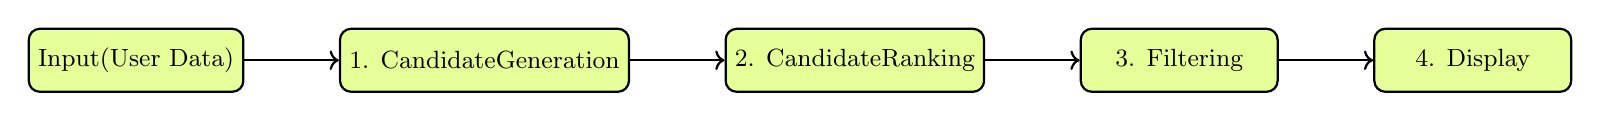
\begin{tikzpicture}[
    node distance=1.4cm and 1.2cm,
    every node/.style={draw, thick, rounded corners, fill=lime!40, minimum width=2.5cm, minimum height=0.8cm, font=\small},
    arrow/.style={->, thick}
]

% Nodes
\node (input) {Input\\(User Data)};
\node (gen) [right=of input] {1. Candidate\\Generation};
\node (rank) [right=of gen] {2. Candidate\\Ranking};
\node (filter) [right=of rank] {3. Filtering};
\node (display) [right=of filter] {4. Display};

% Arrows
\draw[arrow] (input) -- (gen);
\draw[arrow] (gen) -- (rank);
\draw[arrow] (rank) -- (filter);
\draw[arrow] (filter) -- (display);

\end{tikzpicture}
}
\end{center}
\end{frame}


% Architecture of a Top-N Recommender
\begin{frame}{Architecture of a Top-N Recommender}
\begin{center}
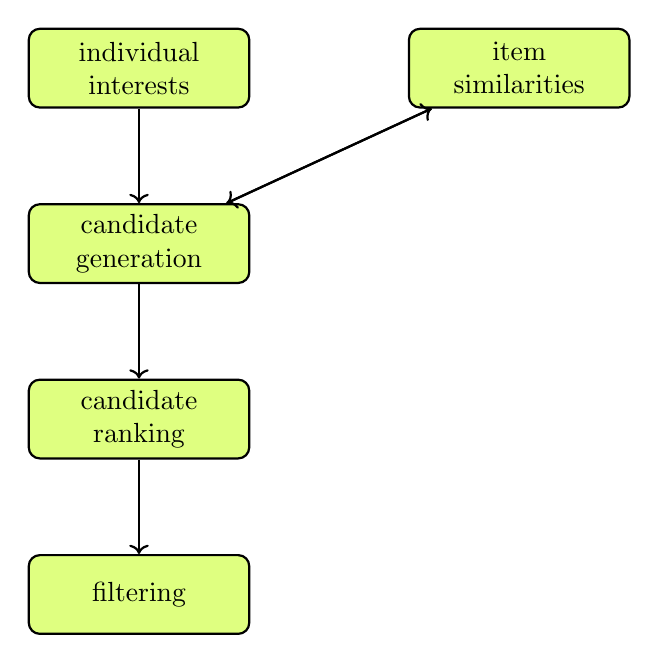
\begin{tikzpicture}[
    every node/.style={draw, thick, align=center, fill=lime!50, rounded corners, minimum width=2.8cm, minimum height=1cm},
    arrow/.style={->, thick},
    node distance=1.2cm and 2cm
]

% Nodes
\node (interests) {individual\\interests};
\node (similarities) [right=of interests] {item\\similarities};
\node (candidates) [below=of interests] {candidate\\generation};
\node (ranking) [below=of candidates] {candidate\\ranking};
\node (filtering) [below=of ranking] {filtering};

% Arrows
\draw[arrow] (interests) -- (candidates);
\draw[arrow] (similarities) -- (candidates);
\draw[arrow] (candidates) -- (similarities);
\draw[arrow] (candidates) -- (ranking);
\draw[arrow] (ranking) -- (filtering);

\end{tikzpicture}
\end{center}
\end{frame}

% Explaining Architecture of a Top-N Recommender
\begin{frame}{Explaining Architecture of a Top-N Recommender}
\begin{itemize}
    \item \textbf{Individual Interests:}  
    User-specific data such as past ratings, purchases, or views. Provides personalized input for recommendations.

    \item \textbf{Item Similarities:}  
    Precomputed relationships between items based on user behavior or content. Learned during preprocessing or training.

    \item \textbf{Candidate Generation:}  
    Uses interests and item similarities to build a shortlist of potentially relevant items for each user.

    \item \textbf{Candidate Ranking:}  
    Scores and ranks the generated candidates using a machine learning model.  
    \textbf{← Training occurs here} — the model learns to predict user preferences based on historical data.

    \item \textbf{Filtering:}  
    Removes items the user has already seen or that don’t meet quality thresholds. Keeps only the Top-N results.
\end{itemize}
\end{frame}


% Old Architecture of a Top-N Recommender
\begin{frame}{Old Architecture of a Top-N Recommender}
\begin{center}
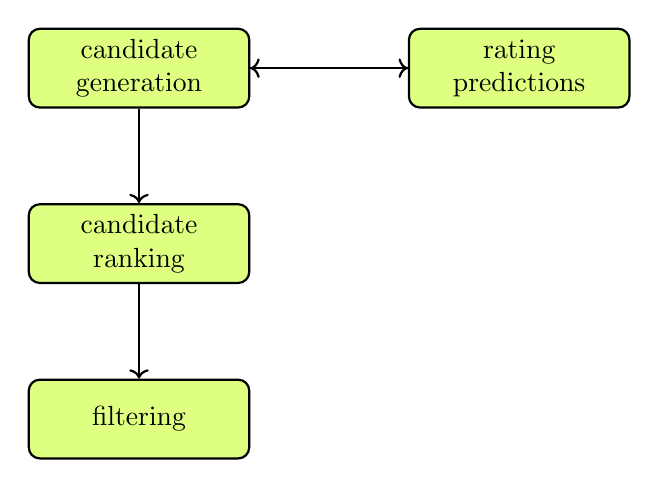
\begin{tikzpicture}[
    every node/.style={draw, thick, align=center, fill=lime!50, rounded corners, minimum width=2.8cm, minimum height=1cm},
    arrow/.style={->, thick},
    node distance=1.2cm and 2cm
]

% Nodes
\node (predictions) {rating\\predictions};
\node (candidates) [left=of predictions] {candidate\\generation};
\node (ranking) [below=of candidates] {candidate\\ranking};
\node (filtering) [below=of ranking] {filtering};

% Arrows
\draw[arrow] (predictions) -- (candidates);
\draw[arrow] (candidates) -- (predictions);
\draw[arrow] (candidates) -- (ranking);
\draw[arrow] (ranking) -- (filtering);

\end{tikzpicture}
\end{center}
\end{frame}

% Explanation of Old Architecture of a Top-N Recommender
\begin{frame}{Explanation of Old Architecture of a Top-N Recommender}
\begin{itemize}
    \item \textbf{Rating Predictions:}  
    A precomputed matrix of predicted ratings for all user-item pairs.  
    These predictions are often generated using matrix factorization or other ML models.  
    \textbf{← Training happens here} — the model is trained to estimate how a user might rate unseen items.

    \item \textbf{Candidate Generation:}  
    Retrieves all predicted ratings for a given user from the prediction matrix.  
    All items are considered candidates.

    \item \textbf{Candidate Ranking:}  
    Sorts candidate items based on predicted ratings to prioritize the most relevant ones.

    \item \textbf{Filtering:}  
    Removes already seen or irrelevant items and limits the output to the Top-N results.
\end{itemize}
\end{frame}


% Slide: Candidate Generation
\begin{frame}{1. Candidate Generation}
\begin{itemize}
    \item Based on the user's previous preferences (e.g., liked Star Trek).
    \item Query a similarity store to find related items (e.g., Star Wars).
    \item Use a distributed store like Cassandra, MongoDB, or Memcached.
    \item Optional: normalize user data (e.g., Z-scores), if sparsity allows.
\end{itemize}
\end{frame}

% Slide: Candidate Scoring
\begin{frame}{Scoring Candidates}
\begin{itemize}
    \item Score items using:
    \begin{itemize}
        \item Original item ratings.
        \item Similarity strength between original and candidate items.
    \end{itemize}
    \item Filter out low-scoring items early.
    \item Assign provisional scores to prepare for ranking.
\end{itemize}
\end{frame}

% Slide: Candidate Ranking
\begin{frame}{2. Candidate Ranking}
\begin{itemize}
    \item Combine scores if items appear via multiple paths.
    \item Boost scores of repeated candidates.
    \item Sort candidates by final score.
    \item Optional: use machine learning (\textbf{learning to rank}) to optimize ranking.
\end{itemize}
\end{frame}

% Slide: Filtering
\begin{frame}{3. Filtering Candidates}
\begin{itemize}
    \item Remove:
    \begin{itemize}
        \item Items already rated/viewed.
        \item Items on a stop-list (e.g., offensive or low-quality).
    \end{itemize}
    \item Apply score thresholds.
    \item Truncate to top $N$ results.
\end{itemize}
\end{frame}

% Slide: Display
\begin{frame}{4. Displaying Results}
\begin{itemize}
    \item The final Top-N list is sent to the UI layer.
    \item Displayed as product/movie/music widgets.
    \item Should feel relevant, fresh, and personalized.
\end{itemize}
\end{frame}

% Slide: Deployment Architecture
\begin{frame}{System Architecture}
\begin{itemize}
    \item Recommendation service is typically distributed and accessed via web APIs.
    \item Key components:
    \begin{itemize}
        \item Interest database (ratings, purchases).
        \item Similarity store (item-item).
        \item Scoring and ranking logic.
        \item Filtering logic.
    \end{itemize}
\end{itemize}
\end{frame}

% Slide: Amazon's Approach
\begin{frame}{Item-Based Collaborative Filtering}
\begin{itemize}
    \item Used by Amazon (2003 paper).
    \item Recommends items similar to those a user liked.
    \item Main challenge: building and maintaining item similarity data.
    \item Simple concept, scalable in practice.
\end{itemize}
\end{frame}

% Slide: Alternative Architecture
% Slide: Alternative Architecture
\begin{frame}{Alternative: Precomputed Rating Predictions}
\begin{itemize}
    \item Build full matrix of predicted ratings for all users and items.
    \item For a user, sort all items by predicted rating → Top-N.
    \item Easier to benchmark prediction accuracy using:
    \begin{itemize}
        \item \textbf{RMSE (Root Mean Square Error):}
        \[
        \text{RMSE} = \sqrt{ \frac{1}{n} \sum_{i=1}^{n} (y_i - x_i)^2 }
        \]
        Penalizes large errors more heavily.
        
        \item \textbf{MAE (Mean Absolute Error):}
        \[
        \text{MAE} = \frac{1}{n} \sum_{i=1}^{n} |y_i - x_i|
        \]
        Treats all errors equally.
    \end{itemize}
    \item \textbf{Drawbacks:}
    \begin{itemize}
        \item Inefficient at runtime (especially for large catalogs).
        \item Doesn’t prioritize known user interests.
    \end{itemize}
\end{itemize}
\end{frame}


% Slide: When to Use Precomputed Ratings
\begin{frame}{When is This Approach OK?}
\begin{itemize}
    \item Acceptable if:
    \begin{itemize}
        \item Item catalog is small.
        \item You want to evaluate rating prediction accuracy.
    \end{itemize}
    \item Still doesn’t align with actual user engagement goals.
    \item Use carefully — may optimize for the wrong thing.
\end{itemize}
\end{frame}

\begin{frame}[plain]
    \begin{center}
        {\LARGE \textbf{Evaluating Recommendations Systems}}
    \end{center}
\end{frame}

\begin{frame}[plain]
    \begin{center}
        {\LARGE \textbf{Train/Test and Cross Validation}}
    \end{center}
\end{frame}

\begin{frame}{Offline Evaluation Methodology}
\begin{itemize}
    \item Recommender systems are trained on prior user behavior to predict preferences.
    \item \textbf{Train/Test Split:}
    \begin{itemize}
        \item Split ratings data into:
        \begin{itemize}
            \item \textbf{Training set} (80–90\% of data).
            \item \textbf{Testing set} (10–20\% of data).
        \end{itemize}
        \item Train the system using only the training data.
        \item Test predictions using the reserved testing data.
    \end{itemize}
\end{itemize}
\end{frame}

% Train/Test Split Graphic
\begin{frame}{Train/Test Split Diagram}
\begin{center}
\resizebox{1.1\textwidth}{!}{%
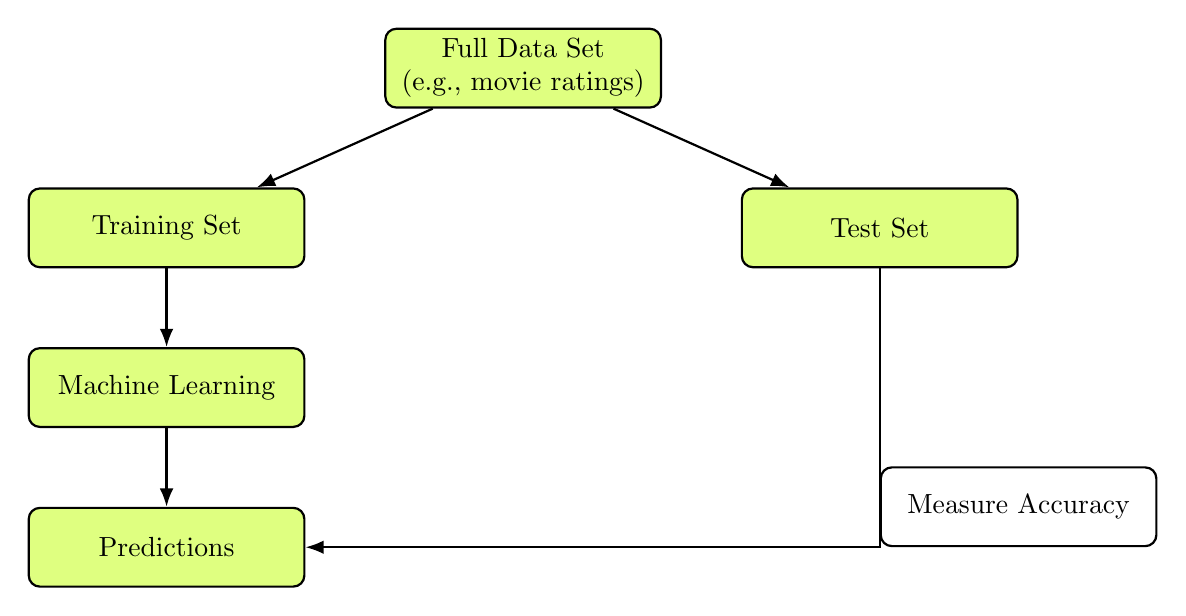
\begin{tikzpicture}[
    node distance=1cm and 1cm,
    align=center,
    every node/.style={draw, thick, rounded corners, minimum width=3.5cm, minimum height=1cm, text centered},
    arrow/.style={-{Latex}, thick}
]

    % Nodes
    \node (full) [fill=lime!50] {Full Data Set \\ (e.g., movie ratings)};
    \node (train) [fill=lime!50, below left=of full] {Training Set};
    \node (test) [fill=lime!50, below right=of full] {Test Set};
    \node (ml) [fill=lime!50, below=of train] {Machine Learning};
    \node (predictions) [fill=lime!50, below=of ml] {Predictions};
    
    % Edges
    \draw [arrow] (full) -- (train);
    \draw [arrow] (full) -- (test);
    \draw [arrow] (train) -- (ml);
    \draw [arrow] (ml) -- (predictions);
    \draw [arrow] (test.south) |- (predictions.east) node[midway, above right] {Measure Accuracy};
\end{tikzpicture}
}
\end{center}
\end{frame}

\begin{frame}{Example of Train/Test Evaluation}
\begin{itemize}
    \item Testing setup:
    \begin{itemize}
        \item User rated the movie "Up" as 5 stars in the test set.
        \item Recommender system predicts the rating without seeing the answer.
    \end{itemize}
    \item Measure how close the prediction is to the real rating.
    \item Repeat across all test set ratings to calculate overall accuracy.
    \item Provides insight into how well the system predicts user ratings.
\end{itemize}
\end{frame}

\begin{frame}{Improving Evaluation: K-Fold Cross-Validation}
\begin{itemize}
    \item An extension of train/test methodology:
    \begin{itemize}
        \item Create multiple randomly assigned training/testing sets (\textbf{folds}).
        \item Train the system on each fold independently.
        \item Measure accuracy for each fold and average the results.
    \end{itemize}
    \item Benefits:
    \begin{itemize}
        \item Reduces the risk of overfitting to a single training set.
        \item Ensures generalizability to different data subsets.
    \end{itemize}
    \item Drawback: Requires significantly more computation.
\end{itemize}
\end{frame}

% K-Fold Cross-Validation Graphic
\begin{frame}{K-Fold Cross-Validation Diagram}
\begin{center}
\resizebox{1.1\textwidth}{!}{%
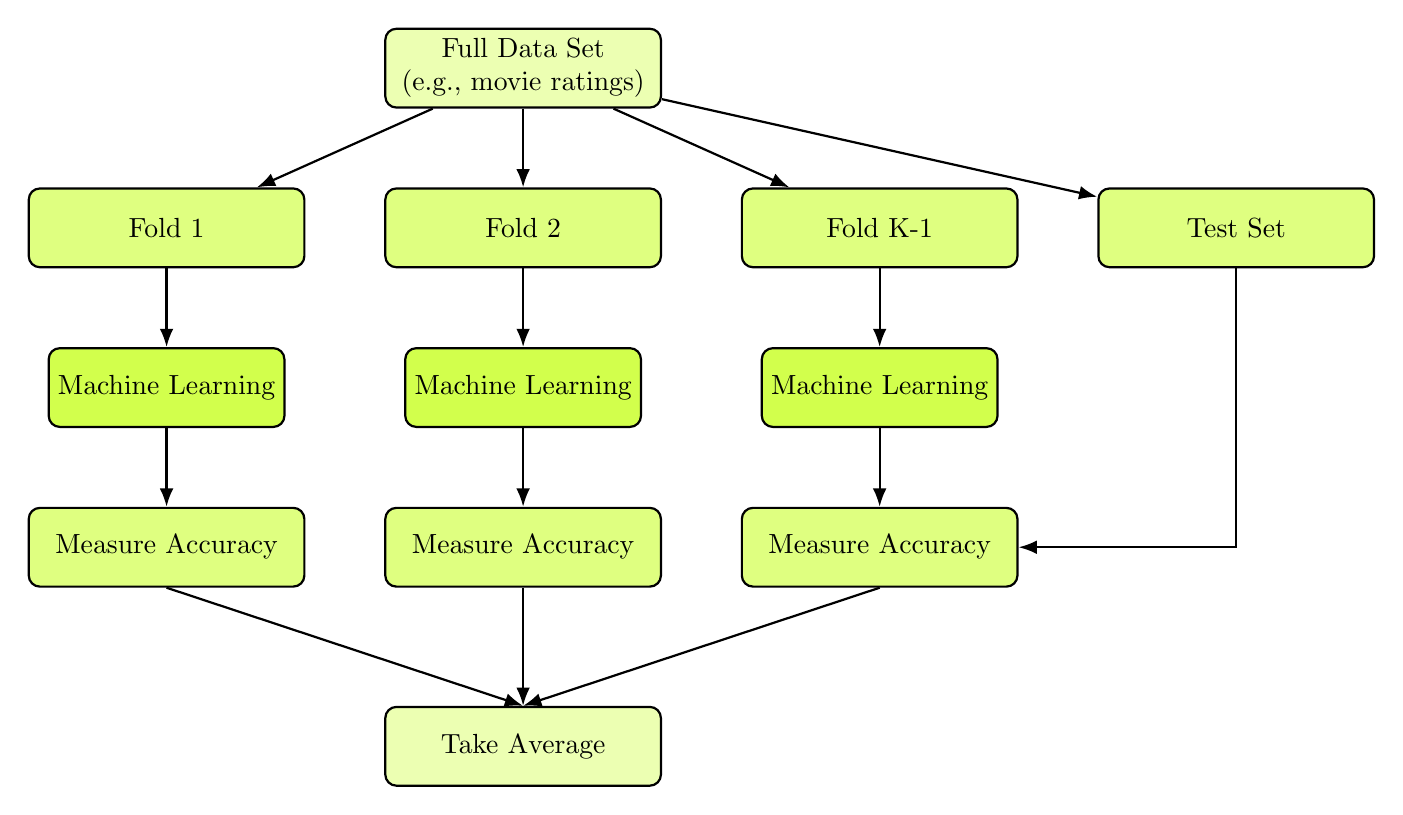
\begin{tikzpicture}[
    node distance=1cm and 1cm,
    align=center,
    every node/.style={draw, thick, rounded corners, minimum width=3.5cm, minimum height=1cm, text centered},
    arrow/.style={-{Latex}, thick}
]

% Nodes
\node (full) [fill=lime!30] {Full Data Set \\ (e.g., movie ratings)};
\node (fold1) [fill=lime!50, below left=of full] {Fold 1};
\node (fold2) [fill=lime!50, right=1cm of fold1] {Fold 2};
\node (foldk1) [fill=lime!50, right=1cm of fold2] {Fold K-1};
\node (test) [fill=lime!50, right=1cm of foldk1] {Test Set};
\node (ml1) [fill=lime!70, below=of fold1, minimum width=2.5cm] {Machine Learning};
\node (ml2) [fill=lime!70, below=of fold2, minimum width=2.5cm] {Machine Learning};
\node (mlk1) [fill=lime!70, below=of foldk1, minimum width=2.5cm] {Machine Learning};
\node (measure1) [fill=lime!50, below=of ml1] {Measure Accuracy};
\node (measure2) [fill=lime!50, below=of ml2] {Measure Accuracy};
\node (measurek1) [fill=lime!50, below=of mlk1] {Measure Accuracy};
\node (average) [fill=lime!30, below=1.5cm of measure2] {Take Average};

% Edges
\draw [arrow] (full) -- (test);
\draw [arrow] (test) |- (measurek1);

\draw [arrow] (full) -- (fold1);
\draw [arrow] (full) -- (fold2);
\draw [arrow] (full) -- (foldk1);
\draw [arrow] (fold1) -- (ml1);
\draw [arrow] (fold2) -- (ml2);
\draw [arrow] (foldk1) -- (mlk1);
\draw [arrow] (ml1) -- (measure1);
\draw [arrow] (ml2) -- (measure2);
\draw [arrow] (mlk1) -- (measurek1);
\draw [arrow] (measure1.south) -- (average.north);
\draw [arrow] (measure2.south) -- (average.north);
\draw [arrow] (measurek1.south) -- (average.north);

\end{tikzpicture}
}
\end{center}
\end{frame}

\begin{frame}{Limitations of Offline Testing}
\begin{itemize}
    \item Train/test and k-fold cross-validation measure:
    \begin{itemize}
        \item How accurately the system predicts ratings for items users already saw.
    \end{itemize}
    \item The goal of recommender systems:
    \begin{itemize}
        \item Recommend new, unseen items that users find interesting.
    \end{itemize}
    \item Fundamental problem:
    \begin{itemize}
        \item Offline methods can’t test the novelty or engagement of recommendations.
        \item Researchers without access to live systems (e.g., Netflix, Amazon) must rely on offline methods.
    \end{itemize}
\end{itemize}
\end{frame}

\begin{frame}[plain]
    \begin{center}
        {\LARGE \textbf{Accuracy Metrics (RMSE, MAE)}}
    \end{center}
\end{frame}

% Slide: Introduction to MAE
\begin{frame}{Mean Absolute Error (MAE)}
\begin{itemize}
    \item MAE is a straightforward metric for evaluating accuracy.
    \item Measures the average absolute error between predicted and actual ratings.
    \item Formula:
\end{itemize}
\[
\text{MAE} = \frac{\sum_{i=1}^{n} \left| y_i - x_i \right|}{n}
\]
\begin{itemize}
    \item \( y_i \): Predicted rating.
    \item \( x_i \): Actual rating.
    \item \( n \): Number of ratings.
\end{itemize}
\end{frame}

% Slide: Example of MAE
\begin{frame}{Example: Calculating MAE}
\begin{itemize}
    \item Let's evaluate a test set with four ratings.
    \item The predicted ratings, actual ratings, and absolute errors are:
\end{itemize}

\begin{center}
\begin{tabular}{|c|c|c|c|}
\hline
\textbf{Predicted Rating} & \textbf{Actual Rating} & \textbf{Error} & \textbf{Absolute Error} \\ \hline
5 & 3 & \( 5 - 3 \) & 2 \\ \hline
4 & 1 & \( 4 - 1 \) & 3 \\ \hline
5 & 4 & \( 5 - 4 \) & 1 \\ \hline
1 & 1 & \( 1 - 1 \) & 0 \\ \hline
\end{tabular}
\end{center}

\begin{itemize}
    \item Sum of absolute errors: \( 2 + 3 + 1 + 0 = 6 \).
    \item MAE: \( \frac{6}{4} = 1.5 \).
\end{itemize}
\end{frame}

% Slide: Introduction to RMSE
\begin{frame}{Root Mean Square Error (RMSE)}
\begin{itemize}
    \item RMSE is another common metric for evaluating accuracy.
    \item Penalizes large errors more than MAE does by squaring the errors.
    \item Formula:
\end{itemize}
\[
\text{RMSE} = \sqrt{\frac{\sum_{i=1}^{n} \left( y_i - x_i \right)^2}{n}}
\]
\begin{itemize}
    \item \( y_i \): Predicted rating.
    \item \( x_i \): Actual rating.
    \item \( n \): Number of ratings.
\end{itemize}
\end{frame}

% Slide: Example of RMSE
\begin{frame}{Example: Calculating RMSE}
\begin{itemize}
    \item Using the same test set as before, let's calculate the squared errors:
\end{itemize}

\begin{center}
\begin{tabular}{|c|c|c|c|}
\hline
\textbf{Predicted Rating} & \textbf{Actual Rating} & \textbf{Error} & \textbf{Squared Error} \\ \hline
5 & 3 & \( 5 - 3 = 2 \) & \( 2^2 = 4 \) \\ \hline
4 & 1 & \( 4 - 1 = 3 \) & \( 3^2 = 9 \) \\ \hline
5 & 4 & \( 5 - 4 = 1 \) & \( 1^2 = 1 \) \\ \hline
1 & 1 & \( 1 - 1 = 0 \) & \( 0^2 = 0 \) \\ \hline
\end{tabular}
\end{center}

\begin{itemize}
    \item Sum of squared errors: \( 4 + 9 + 1 + 0 = 14 \).
    \item RMSE: \( \sqrt{\frac{14}{4}} \approx 1.87 \).
\end{itemize}
\end{frame}

% Slide: MAE vs. RMSE
\begin{frame}{MAE vs. RMSE}
\begin{itemize}
    \item MAE treats all errors equally.
    \item RMSE penalizes large errors more heavily.
    \item RMSE is higher than MAE when large errors are present.
\end{itemize}

\begin{itemize}
    \item For our example:
    \begin{itemize}
        \item MAE: \( 1.5 \).
        \item RMSE: \( 1.87 \).
    \end{itemize}
\end{itemize}
\end{frame}

% Slide: Real-World Metrics
\begin{frame}{Real-World Metrics}
\begin{itemize}
    \item Users care about the quality of recommendations, not prediction accuracy.
    \item Top-N recommendation lists are more relevant in practice:
    \begin{itemize}
        \item How likely are users to interact with recommended items?
        \item Do recommendations help users discover new content?
    \end{itemize}
    \item Offline metrics like MAE and RMSE are useful for development but limited in scope.
\end{itemize}
\end{frame}

\begin{frame}[plain]
    \begin{center}
        {\LARGE \textbf{Top-N Hit Rate - Ways}}
    \end{center}
\end{frame}

% Slide: Hit Rate Introduction
\begin{frame}{Hit Rate (HR)}
\begin{itemize}
    \item Top-N means the system picks the best N recommendations (like top 5 or top 10) that it thinks a user will like the most
    \item Hit rate measures the success of a recommender system in generating Top-N recommendations.
    \item If one of the recommendations in a user’s Top-N list matches an item they actually rated, it’s considered a "hit."
    \item Formula:
\end{itemize}
\[
\text{Hit Rate} = \frac{\text{Hits}}{\text{Users}}
\]
\begin{itemize}
    \item Hits: Number of successfully recommended items.
    \item Users: Total number of users.
\end{itemize}
\end{frame}

% Slide: Example of Hit Rate
\begin{frame}{Example: Hit Rate}
\begin{itemize}
    \item Let’s consider a test set of Top-N recommendations.
    \item If a user rates at least one of the recommended items, it’s counted as a "hit."
    \item Example calculation:
\end{itemize}

\begin{center}
\begin{tabular}{|c|c|}
\hline
\textbf{User} & \textbf{Hit (Yes/No)} \\ \hline
User 1 & Yes \\ \hline
User 2 & No \\ \hline
User 3 & Yes \\ \hline
User 4 & Yes \\ \hline
\end{tabular}
\end{center}

\begin{itemize}
    \item Total Hits = 3, Total Users = 4.
    \item Hit Rate = \( \frac{3}{4} = 0.75 \) or 75\%.
\end{itemize}
\end{frame}

% Slide: Average Reciprocal Hit Rate
\begin{frame}{Average Reciprocal Hit Rate (ARHR)}
\begin{itemize}
    \item ARHR builds on hit rate but accounts for the position of hits in the Top-N list.
    \item Formula:
\end{itemize}
\[
\text{ARHR} = \frac{\sum_{i=1}^{n} \frac{1}{\text{rank}_i}}{\text{Users}}
\]
\begin{itemize}
    \item \( \text{rank}_i \): Rank position of the hit.
    \item Users: Total number of users.
\end{itemize}

\begin{itemize}
    \item Hits near the top of the list (e.g., rank 1) are weighted more heavily than hits at the bottom.
\end{itemize}
\end{frame}

% Slide: Example of ARHR
\begin{frame}{Example: ARHR Calculation}
\begin{itemize}
    \item Consider the following example with three hits:
\end{itemize}

\begin{center}
\begin{tabular}{|c|c|}
\hline
\textbf{Rank} & \textbf{Reciprocal Rank} \\ \hline
1 & \( \frac{1}{1} = 1.0 \) \\ \hline
2 & \( \frac{1}{2} = 0.5 \) \\ \hline
3 & \( \frac{1}{3} = 0.33 \) \\ \hline
\end{tabular}
\end{center}

\begin{itemize}
    \item ARHR = \( \frac{1.0 + 0.5 + 0.33}{3} \approx 0.61 \).
\end{itemize}
\end{frame}

% Slide: Cumulative Hit Rate
\begin{frame}{Cumulative Hit Rate (cHR)}
\begin{itemize}
    \item A variation of hit rate that filters hits based on a rating threshold.
    \item Only hits above a certain predicted or actual rating threshold are counted.
    \item Example:
\end{itemize}

\begin{center}
\begin{tabular}{|c|c|}
\hline
\textbf{Hit Rank} & \textbf{Predicted Rating} \\ \hline
1 & 5.0 \\ \hline
2 & 3.0 \\ \hline
3 & 5.0 \\ \hline
4 & 2.0 \\ \hline
\end{tabular}
\end{center}

\begin{itemize}
    \item If the threshold is \( \geq 3.0 \), we exclude hits with predicted ratings below 3.0.
    \item Adjusted cHR = \( \frac{\text{Filtered Hits}}{\text{Users}} \).
\end{itemize}
\end{frame}

% Slide: Cumulative Hit Rate Formula
\begin{frame}{Cumulative Hit Rate (cHR) - Formula}
\begin{itemize}
    \item \textbf{Definition:} Measures hit rate while excluding low-confidence or low-rating predictions.
    \item \textbf{Formula:}
    \[
    \text{cHR} = \frac{\text{Number of Hits with Rating} \geq \text{Threshold}}{\text{Total Users}}
    \]
    \item Encourages recommending items the model believes the user will rate highly.
\end{itemize}
\end{frame}

% Slide: Cumulative Hit Rate Example
\begin{frame}{Example: Cumulative Hit Rate Calculation}
\begin{itemize}
    \item Assume rating threshold = 3.0
\end{itemize}
\begin{center}
\begin{tabular}{|c|c|}
\hline
\textbf{Hit Rank} & \textbf{Predicted Rating} \\ \hline
1 & 5.0 \\ \hline
2 & 3.0 \\ \hline
3 & 5.0 \\ \hline
4 & 2.0 \\ \hline
\end{tabular}
\end{center}
\vspace{0.5em}
\begin{itemize}
    \item Filtered Hits = 3 (ratings 5.0, 3.0, 5.0)
    \item Total Users = 4
    \item \textbf{cHR = \( \frac{3}{4} = 0.75 \) or 75\%}
\end{itemize}
\end{frame}

% Slide: Rating Hit Rate
\begin{frame}{Rating Hit Rate (rHR)}
\begin{itemize}
    \item \textbf{Definition:} Analyzes hit rate across different predicted rating bins.
    \item \textbf{Formula:}
    \[
    \text{rHR}_r = \frac{\text{Number of Hits with Predicted Rating } r}{\text{Total Users}}
    \]
    \item Breaks down hit rates by predicted rating score.
    \item Helps understand the distribution of predicted ratings for successful recommendations.
    \item Example:
\end{itemize}

\begin{center}
\begin{tabular}{|c|c|}
\hline
\textbf{Rating} & \textbf{Hit Rate} \\ \hline
5.0 & \( 0.001 \) \\ \hline
4.0 & \( 0.004 \) \\ \hline
3.0 & \( 0.030 \) \\ \hline
2.0 & \( 0.001 \) \\ \hline
1.0 & \( 0.0005 \) \\ \hline
\end{tabular}
\end{center}
\end{frame}

\begin{frame}[plain]
    \begin{center}
        {\LARGE \textbf{Converge, Diversity and Novelty}}
    \end{center}
\end{frame}

% Slide: Introduction to Coverage
\begin{frame}{Coverage}
\begin{itemize}
    \item \textbf{Definition:} Coverage measures the percentage of user-item pairs that your system can make predictions for.
    \item Formula:
    \[
    \text{Coverage} = \frac{\text{Predicted User-Item Pairs}}{\text{Total Possible User-Item Pairs}}
    \]
    \item High coverage ensures that more items and users are included in the recommendation process.
    \item Tradeoff: Higher coverage might reduce accuracy.
\end{itemize}
\end{frame}

% Example: Calculating Coverage
\begin{frame}{Example: Calculating Coverage}
\begin{itemize}
    \item Suppose we have:
    \begin{itemize}
        \item 5 users.
        \item 6 items.
        \item Total possible user-item pairs: \( 5 \times 6 = 30 \).
        \item Model predicts ratings for 18 of those pairs.
    \end{itemize}
\end{itemize}

\begin{block}{Coverage Formula}
\[
\text{Coverage} = \frac{18}{30} = 0.6 \text{ or } 60\%
\]
\end{block}

\begin{itemize}
    \item The recommender covers 60\% of the user-item space.
    \item Higher coverage ensures broader personalization, but may impact accuracy.
\end{itemize}
\end{frame}

% Slide: Item Similarity
\begin{frame}{Item Similarity}
\begin{itemize}
    \item Similarity quantifies how closely two items are related based on user behavior.
    \item Commonly used to recommend items similar to those a user liked.
    \item Types of similarity:
    \begin{itemize}
        \item \textbf{Cosine similarity}: Angle between rating vectors.
        \item \textbf{Pearson correlation}: Measures linear correlation.
    \end{itemize}
    \item Similarity is usually computed using rating vectors for items across users.
\end{itemize}
\end{frame}

% Slide: Example: Cosine Similarity
\begin{frame}{Example: Calculating Cosine Similarity}
\begin{itemize}
    \item Ratings from 3 users for two items:
\end{itemize}

\begin{center}
\begin{tabular}{|c|c|c|}
\hline
\textbf{User} & \textbf{Item A} & \textbf{Item B} \\ \hline
User 1 & 5 & 3 \\ \hline
User 2 & 4 & 2 \\ \hline
User 3 & 0 & 2 \\ \hline
\end{tabular}
\end{center}

\begin{itemize}
    \item Cosine similarity formula:
    \[
    \text{sim}(A,B) = \frac{\vec{A} \cdot \vec{B}}{||\vec{A}|| \times ||\vec{B}||}
    \]
    \item Vectors:
    \[
    \vec{A} = [5, 4, 0], \quad \vec{B} = [3, 2, 2]
    \]
    \item Result:
    \[
    \text{sim}(A,B) \approx 0.76
    \]
\end{itemize}
\end{frame}


% Slide: Diversity
\begin{frame}{Diversity}
\begin{itemize}
    \item \textbf{Definition:} Diversity measures how varied the recommendations are within the Top-N list.
    \item Calculated using average similarity \( S \) between recommended items:
    \[
    \text{Diversity} = 1 - S
    \]
    \item \( S \): Average similarity between item pairs in the recommendation list.
    \item High diversity may lead to novel recommendations but risks reducing relevance.
\end{itemize}
\end{frame}

% Slide: Example of Diversity
\begin{frame}{Example: Calculating Diversity}
\begin{itemize}
    \item Example similarity scores between items in a Top-N list:
\end{itemize}
\begin{center}
\begin{tabular}{|c|c|c|}
\hline
\textbf{Item Pair} & \textbf{Similarity} \\ \hline
Item 1, Item 2 & 0.7 \\ \hline
Item 2, Item 3 & 0.8 \\ \hline
Item 3, Item 1 & 0.6 \\ \hline
\end{tabular}
\end{center}
\begin{itemize}
    \item Average similarity \( S = \frac{0.7 + 0.8 + 0.6}{3} = 0.7 \).
    \item Diversity \( = 1 - 0.7 = 0.3 \).
\end{itemize}
\end{frame}

% Slide: Novelty
\begin{frame}{Novelty}
\begin{itemize}
    \item \textbf{Definition:} Measures how "unpopular" the recommended items are.
    \item Computed as the mean popularity rank of the recommended items.
\end{itemize}

\[
\text{Novelty} = \frac{1}{N} \sum_{i=1}^{N} \text{rank}(i)
\]

\begin{itemize}
    \item \textbf{N}: Total number of recommended items in the Top-N list.
    \item \textbf{rank(i)}: Popularity rank of item \( i \) (higher = less popular).
    \item Higher novelty → more obscure items are being recommended.
    \item Tradeoff: Too much novelty can harm relevance and trust.
\end{itemize}
\end{frame}


% Example: Calculating Novelty
\begin{frame}{Example: Calculating Novelty}
\begin{itemize}
    \item Assume a Top-5 recommendation list for a user:
\end{itemize}

\begin{center}
\begin{tabular}{|c|c|}
\hline
\textbf{Item} & \textbf{Popularity Rank} \\ \hline
Item A & 45 \\ \hline
Item B & 120 \\ \hline
Item C & 230 \\ \hline
Item D & 310 \\ \hline
Item E & 400 \\ \hline
\end{tabular}
\end{center}

\begin{block}{Novelty Formula}
\[
\text{Novelty} = \frac{45 + 120 + 230 + 310 + 400}{5} = 221
\]
\end{block}

\begin{itemize}
    \item Higher mean rank → less popular items → more novelty.
    \item Promotes long-tail discovery, but too much may harm user trust.
\end{itemize}
\end{frame}


% % Slide: Long Tail
\begin{frame}{The Long Tail Effect}
\begin{itemize}
    \item Popularity of items often follows a "long tail" distribution:
    \begin{itemize}
        \item Few items are very popular (head).
        \item Most items have low demand (long tail).
    \end{itemize}
    \item Recommender systems surface niche, less popular items in the long tail.
    \item Benefits:
    \begin{itemize}
        \item Users discover new interests.
        \item Lesser-known items get more exposure.
    \end{itemize}
\end{itemize}
\end{frame}

% % Slide: Long Tail
\begin{frame}{The Long Tail Effect}
\begin{center}
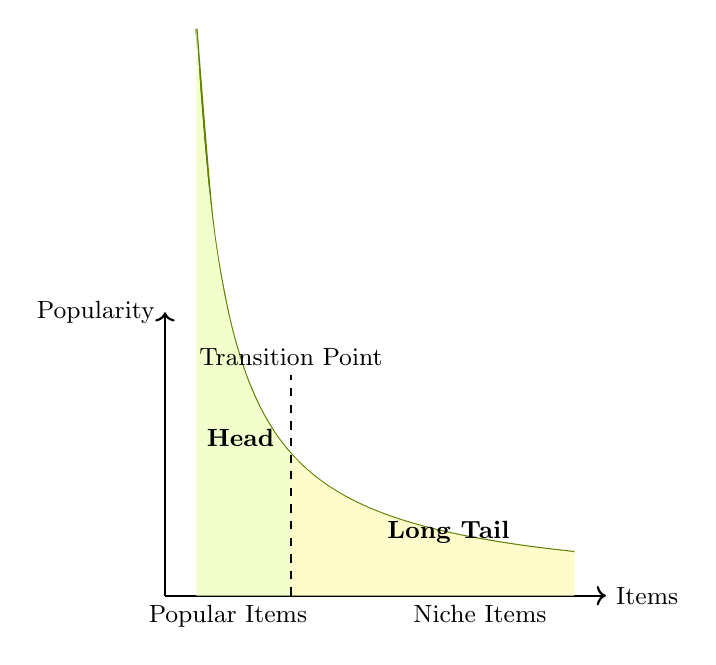
\begin{tikzpicture}[scale=0.8, every node/.style={font=\small}]
    % Axes
    \draw[->, thick] (0, 0) -- (7, 0) node[right] {Items};
    \draw[->, thick] (0, 0) -- (0, 4.5) node[left] {Popularity};

    % Curve
    \draw[thick, lime!50!black, smooth, domain=0.5:6.5] plot (\x, {4.5 / (\x)});

    % Highlighted Areas
    \fill[lime!20] (0.5, 0) -- plot[domain=0.5:2] (\x, {4.5 / (\x)}) -- (2, 0) -- cycle;
    \fill[yellow!20] (2, 0) -- plot[domain=2:6.5] (\x, {4.5 / (\x)}) -- (6.5, 0) -- cycle;

    % Labels
    \node at (1.2, 2.5) {\textbf{Head}};
    \node at (4.5, 1) {\textbf{Long Tail}};
    \draw[dashed] (2, 0) -- (2, 3.5) node[above] {Transition Point};

    % Additional Explanations
    \node[below] at (1, 0) {Popular Items};
    \node[below] at (5, 0) {Niche Items};
\end{tikzpicture}
\end{center}
\end{frame}

% % Slide: Striking a Balance
\begin{frame}{Balancing Metrics in Recommender Systems}
\begin{itemize}
    \item Recommender systems require a balance between:
    \begin{itemize}
        \item Familiar, popular items (trust-building).
        \item Novel, diverse items (serendipitous discovery).
    \end{itemize}
    \item Metrics such as coverage, diversity, and novelty are interdependent:
    \begin{itemize}
        \item Increasing one might reduce another.
        \item The right balance depends on your use case and audience.
    \end{itemize}
\end{itemize}
\end{frame}

\begin{frame}[plain]
    \begin{center}
        {\LARGE \textbf{Churn, Responsiveness and A/B Tests}}
    \end{center}
\end{frame}

% % Slide: Churn
\begin{frame}{Churn}
\begin{itemize}
    \item \textbf{Definition:} Measures how often recommendations for a user change.
    \item \textbf{Purpose:} Indicates how sensitive a system is to new user behavior.
    \item High churn can indicate:
    \begin{itemize}
        \item System responsiveness to user updates.
        \item Over-sensitivity to minor user actions.
    \end{itemize}
    \item Tradeoff: High churn risks showing irrelevant or overly dynamic recommendations.
\end{itemize}
\end{frame}

% % Slide: Example of Churn
\begin{frame}{Example: Churn}
\begin{itemize}
    \item Suppose a user rates a new movie:
    \begin{itemize}
        \item Does this substantially change their recommendations?
        \item High churn indicates recommendations update drastically.
    \end{itemize}
    \item Balance required: Randomization can keep recommendations fresh but may reduce relevance.
\end{itemize}
\end{frame}

% % Slide: Responsiveness
\begin{frame}{Responsiveness}
\begin{itemize}
    \item \textbf{Definition:} Measures how quickly new user behavior influences recommendations.
    \item \textbf{Purpose:} Ensures that recommendations adapt to user updates efficiently.
    \item Levels of responsiveness:
    \begin{itemize}
        \item \textbf{Immediate:} Recommendations change instantly after user actions.
        \item \textbf{Delayed:} Recommendations update after periodic data processing.
    \end{itemize}
    \item Tradeoff: Higher responsiveness increases system complexity and maintenance costs.
\end{itemize}
\end{frame}

% % Slide: Balancing Metrics
\begin{frame}{Balancing Metrics}
\begin{itemize}
    \item Offline metrics include:
    \begin{itemize}
        \item MAE, RMSE.
        \item Hit Rate, Diversity, Novelty, Coverage.
        \item Churn, Responsiveness.
    \end{itemize}
    \item Tradeoffs between metrics:
    \begin{itemize}
        \item High diversity may reduce relevance.
        \item High churn may reduce user trust.
        \item High novelty may overwhelm users with unfamiliar options.
    \end{itemize}
    \item The balance depends on business goals and cultural context.
\end{itemize}
\end{frame}

% % Slide: Online A/B Testing
\begin{frame}{Online A/B Testing}
\begin{itemize}
    \item \textbf{Definition:} Tests recommendations on real users to measure their actual reactions.
    \item \textbf{Process:}
    \begin{itemize}
        \item Split users into groups.
        \item Show different recommendation algorithms to each group.
        \item Measure engagement, purchases, or clicks.
    \end{itemize}
    \item \textbf{Benefits:}
    \begin{itemize}
        \item Ensures recommendations work in real-world scenarios.
        \item Avoids introducing unnecessary complexity.
    \end{itemize}
\end{itemize}
\end{frame}

% Slide: Perceived Quality
\begin{frame}{Perceived Quality of Recommendations}
\begin{itemize}
    \item Users can explicitly rate the quality of recommendations.
    \item Challenges:
    \begin{itemize}
        \item Users may confuse rating the item with rating the recommendation.
        \item Requires additional user effort with little perceived benefit.
        \item Data collected may be sparse and unclear.
    \end{itemize}
    \item Best practice: Focus on user engagement and A/B tests instead.
\end{itemize}
\end{frame}

\begin{frame}[plain]
    \begin{center}
        {\LARGE \textbf{Evaluation with python code}}
    \end{center}
\end{frame}

% Evaluation
\begin{frame}{Evaluation}
\begin{itemize}
    \item The \textbf{MovieLens.py} file defines a \textbf{MovieLens} class that loads and parses the dataset.
    
    \item The \textbf{RecommenderMetrics.py} file defines a \textbf{RecommenderMetrics} class that calculates the following metrics:
    \begin{itemize}
        \item MAE (Mean Absolute Error)
        \item RMSE (Root Mean Squared Error)
        \item GetTopN
        \item HitRate
        \item CumulativeHitRate (cHR)
        \item RatingHitRate (rHR)
        \item AverageReciprocalHitRank (ARHR)
        \item UserCoverage
        \item Diversity
        \item Novelty
    \end{itemize}

    \item The \textbf{TestMetrics.py} file uses these two classes to load the data, compute all metrics, and print the evaluation results.
\end{itemize}
\end{frame}

% \begin{frame}[plain]
%     \begin{center}
%         {\LARGE \textbf{Framework}}
%     \end{center}
% \end{frame}

% % % Slide: Intro to Framework
% \begin{frame}{Recommender System Framework}
%     \begin{itemize}
%         \item Evaluating and comparing recommender algorithms is a core goal.
%         \item Built on top of \textbf{SurpriseLib}.
%         \item Framework structure:
%         \begin{itemize}
%             \item EvaluationData: Prepares data splits.
%             \item EvaluatedAlgorithm: Wraps algorithms for evaluation.
%             \item Evaluator: Compares algorithms using defined metrics.
%         \end{itemize}
%         \item Supports offline evaluation using RMSE, MAE, Hit Rate, etc.
%     \end{itemize}
% \end{frame}


% % % Slide: Surpriselib Base Class
% \begin{frame}{SurpriseLib Algorithm Base Class}
%     \begin{center}
%     \resizebox{1.0\textwidth}{!}{%
%         \begin{tikzpicture}[
%             node distance=1.5cm and 2.5cm,
%             every node/.style={draw, thick, rounded corners, minimum width=2.5cm, minimum height=0.75cm, align=center, fill=lime!50},
%             arrow/.style={-{Latex}, thick},
%         ]
%             % Nodes
%             \node (AlgoBase) [fill=lime!30] {AlgoBase};
%             \node (SVD) [fill=lime!50, below left=of AlgoBase] {SVD};
%             \node (KNNBasic) [fill=lime!50, right=1cm of SVD] {KNNBasic};
%             \node (SVDpp) [fill=lime!50, right=1cm of KNNBasic] {SVDpp};
%             \node (Custom) [fill=lime!50, right=1cm of SVDpp] {Custom};

%             % Edges
%             \draw [arrow] (AlgoBase) -- (SVD);
%             \draw [arrow] (AlgoBase) -- (KNNBasic);
%             \draw [arrow] (AlgoBase) -- (SVDpp);
%             \draw [arrow] (AlgoBase) -- (Custom);
%         \end{tikzpicture}
%     }
%     \end{center}
%     \begin{itemize}
%         \item AlgoBase defines consistent interfaces like \texttt{fit} and \texttt{test}.
%         \item Allows creating custom algorithms for flexibility.
%     \end{itemize}
% \end{frame}

% % Slide: Creating Custom Algorithm
% \begin{frame}{Creating a Custom Algorithm}
%     \begin{itemize}
%         \item Define a new class inheriting from \texttt{AlgoBase}.
%         \item Implement the \texttt{estimate()} function to predict ratings.
%         \item Example:
%     \end{itemize}

%     {\small
%     \begin{flushleft}
% \texttt{class MyOwnAlgorithm(AlgoBase):} \\
% \hspace*{1em}\texttt{def \_\_init\_\_(self):} \\
% \hspace*{2em}\texttt{AlgoBase.\_\_init\_\_(self)} \\
% \hspace*{1em}\texttt{def estimate(self, user, item):} \\
% \hspace*{2em}\texttt{return 3}
%     \end{flushleft}
%     }

%     \begin{itemize}
%         \item Simple logic: Predicts a rating of 3 for all items and users.
%         \item Customization allows tailored recommendation strategies.
%     \end{itemize}
% \end{frame}


% % Slide: Building on Top of SurpriseLib
% \begin{frame}{Building on Top of SurpriseLib}
%     \begin{center}
%         \begin{tikzpicture}[
%             node distance=1.5cm and 1.5cm,
%             every node/.style={draw, thick, rounded corners, minimum width=3.0cm, minimum height=0.75cm, align=center, fill=lime!50},
%             arrow/.style={-{Latex}, thick},
%         ]
%             % Nodes
%             \node (EA) {EvaluatedAlgorithm (AlgoBase)};
%             \node (ED) [right=of EA] {EvaluationData (Dataset)};
%             \node (Metrics) [below=of EA] {RecommenderMetrics};

%             % Edges
%             \draw [arrow] (EA) -- (ED);
%             \draw [arrow] (ED) -- (Metrics);
%         \end{tikzpicture}
%     \end{center}
%     \begin{itemize}
%         \item \textbf{EvaluatedAlgorithm:} Measures accuracy, hit rate, coverage, diversity, etc.
%         \item \textbf{EvaluationData:} Prepares train/test splits for evaluation.
%     \end{itemize}
% \end{frame}

% % % Slide: Algorithm Bake-Offs
% \begin{frame}{Algorithm Bake-Offs}
%     \begin{itemize}
%         \item Use \texttt{Evaluator} to compare multiple algorithms.
%         \item \textbf{Key Functions:}
%         \begin{itemize}
%             \item \texttt{AddAlgorithm(algorithm):} Add algorithm for comparison.
%             \item \texttt{Evaluate():} Run all metrics and compare results.
%         \end{itemize}
%     \end{itemize}

%     {\small
%     \begin{flushleft}
% \texttt{\# Example} \\
% \texttt{evaluator = Evaluator(evaluationData)} \\
% \texttt{evaluator.AddAlgorithm(SVD(), "SVD")} \\
% \texttt{evaluator.AddAlgorithm(Random(), "Random")} \\
% \texttt{evaluator.Evaluate()}
%     \end{flushleft}
%     }

%     \begin{itemize}
%         \item Minimal code for evaluating and comparing algorithms.
%     \end{itemize}
% \end{frame}

% % % Slide: Evaluation Metrics
% \begin{frame}{Evaluation Metrics Overview}
%     \begin{itemize}
%         \item \textbf{RMSE:} Penalizes large errors.
%         \[
%         RMSE = \sqrt{\frac{1}{n} \sum_{i=1}^{n} (y_i - x_i)^2}
%         \]
%         \item \textbf{MAE:} Mean of absolute errors.
%         \[
%         MAE = \frac{1}{n} \sum_{i=1}^{n} |y_i - x_i|
%         \]
%         \item \textbf{Hit Rate:} Proportion of successful top-N recommendations.
%         \item \textbf{Diversity:} Measures variety of recommendations.
%         \[
%         Diversity = 1 - S
%         \]
%     \end{itemize}
% \end{frame}

% % Slide: Results Interpretation
% \begin{frame}{Results Interpretation}
%     \begin{itemize}
%         \item RMSE: 0.9, MAE: 0.7 — Acceptable accuracy for small datasets.
%         \item Hit Rate: 3\% — Decent for testing with limited data.
%         \item Diversity: 0.96 — Recommends many niche items.
%         \item Novelty: Deep into the long tail (avg. rank = 491).
%         \item \textbf{Takeaway:} Results are acceptable for offline testing but might not generalize to online scenarios.
%     \end{itemize}
% \end{frame}

% % Slide: Final Thoughts
% \begin{frame}{Final Thoughts}
%     \begin{itemize}
%         \item A robust framework simplifies algorithm evaluation.
%         \item Offline metrics are valuable but not definitive.
%         \item Online A/B testing is the ultimate measure of success.
%         \item The framework enables rapid experimentation and iteration.
%     \end{itemize}
% \end{frame}

% ------------------------------------------------------------------------
\begin{frame}[plain]
    \begin{center}
        {\LARGE \textbf{Content-Based Filtering}}
    \end{center}
\end{frame}

% ------------------------------------------------------------------------
\begin{frame}{Introduction to Content-Based Filtering}
\begin{itemize}
  \item Recommend items based solely on their own attributes.
  \item Useful when collaborative data is scarce or as a hybrid enhancement.
  \item Example: Suggest movies in the same genre and release period as ones a user enjoyed.
\end{itemize}
\end{frame}

% ------------------------------------------------------------------------
\begin{frame}{MovieLens Genre Data}
\begin{itemize}
  \item Each movie record lists its genres, e.g., Adventure|Comedy|Fantasy.
  \item There are 18 possible genres per movie.
\end{itemize}
\begin{center}
\scriptsize
\resizebox{1.09\textwidth}{!}{
\begin{tabular}{rl l}
\textbf{ID} & \textbf{Title} & \textbf{Genres} \\ \hline
1 & Toy Story (1995)                & Adventure|Animation|Children|Comedy|Fantasy \\
2 & Jumanji (1995)                  & Adventure|Children|Fantasy            \\
3 & Grumpier Old Men (1995)         & Comedy|Romance                        \\
4 & Waiting to Exhale (1995)        & Comedy|Drama|Romance                  \\
5 & Father of the Bride Part II (95)& Comedy                                \\
\end{tabular}
}
\end{center}
\end{frame}

% ------------------------------------------------------------------------
\begin{frame}{Genres as Binary Vectors}
\begin{itemize}
  \item Convert each genre list into an 18-dimensional \{0,1\} vector.
  \item 1 indicates presence of a genre, 0 absence.
\end{itemize}
\begin{center}
\scriptsize
\resizebox{1.09\textwidth}{!}{
\begin{tabular}{l|*{10}{c}|c}
Movie            & Action & Adventure & Animation & Children & Comedy & \dots & Romance & Sci-Fi & Thriller & Western \\ \hline
Toy Story        & 0 & 1 & 1 & 1 & 1 & \dots & 0 & 0 & 0 & 0 \\
Jumanji          & 0 & 1 & 0 & 1 & 0 & \dots & 0 & 0 & 0 & 0 \\
Grumpier Old Men & 0 & 0 & 0 & 0 & 1 & \dots & 1 & 0 & 0 & 0 \\
\end{tabular}
}
\end{center}
\end{frame}


% ------------------------------------------------------------------------
\begin{frame}{Cosine Similarity (2D Illustration)}
\begin{center}
\begin{tikzpicture}[scale=1, every node/.style={font=\small},
    axis/.style={->, thick, gray},
    sim/.style={very thick, LimeGreen},
    vec/.style={thick, gray!70},
    proj/.style={thick, ForestGreen},
    anglearc/.style={thick, Orchid}
]

  % Left: Movie genre vector space
  % axes
  \draw[axis] (0,0) -- (3,0) node[right] {Comedy};
  \draw[axis] (0,0) -- (0,3) node[above] {Adventure};

  % Indiana Jones vector (adventure only)
  \coordinate (IJ) at (0,2);
  \draw[vec] (0,0) -- (IJ)
    node[midway, above left] {\includegraphics[height=0.8cm]{indiana.png}};

  % Toy Story vector (both comedy & adventure)
  \coordinate (TH) at (2,2);
  \draw[sim] (0,0) -- (TH)
    node[midway, above right] {\includegraphics[height=0.8cm]{toy_story.png}};

  % Grumpier Old Men vector (comedy only)
  \coordinate (GO) at (2,0);
  \draw[sim] (0,0) -- (GO)
    node[midway, below] {\includegraphics[height=0.8cm]{grumpier.png}};

  % Angle θ
  \draw[anglearc, ->] (0.8,0) arc[start angle=0,end angle=45,radius=0.8];
  \node[Orchid] at (1.05,0.2) {\scriptsize $\theta$};

  % Right: Unit circle diagram
  \begin{scope}[xshift=6.5cm, yshift=1cm, scale=1.5]
    % Circle and axes
    \draw[gray, thick] (0,0) circle(1);
    \draw[axis] (-1.2,0) -- (1.2,0);
    \draw[axis] (0,-1.2) -- (0,1.2);

    % Vector at 45 degrees (cosθ, sinθ)
    \coordinate (V) at ({cos(45)},{sin(45)});
    \coordinate (H) at ({cos(45)}, 0);

    % Vector and projections
    \draw[sim] (0,0) -- (V) node[above right] {\footnotesize 1};
    \draw[proj] (0,0) -- (H) node[midway, below] {\scriptsize $\cos\theta$};
    \draw[proj] (H) -- (V) node[midway, right] {\scriptsize $\sin\theta$};

    % Angle
    \draw[anglearc, ->] (0.2,0) arc[start angle=0,end angle=45,radius=0.2];
    \node[Orchid] at (0.28,0.08) {\scriptsize $\theta$};
  \end{scope}

\end{tikzpicture}
\end{center}
\end{frame}

% ------------------------------------------------------------------------
\begin{frame}{Cosine Similarity: Measuring Genre-Based Movie Similarity}
\begin{itemize}
    \item This diagram explains how we compute similarity between movies using genre attributes.
    \item Each axis represents a binary genre feature — here simplified to just two: \textbf{Comedy} and \textbf{Adventure}.
    \item Movies are plotted as vectors in this genre space:
    \begin{itemize}
        \item \textbf{Toy Story} and \textbf{Monty Python} are both comedy \& adventure → vector (1,1).
        \item \textbf{Grumpier Old Men} is only comedy → vector (1,0).
        \item \textbf{Indiana Jones} is only adventure → vector (0,1).
    \end{itemize}
    \item The angle \(\theta\) between vectors reflects their similarity. The \textbf{cosine of that angle} gives us:
    \[
    \text{cosine similarity} = \frac{\vec{x} \cdot \vec{y}}{\|\vec{x}\| \cdot \|\vec{y}\|}
    \]
    \item Interpretation:
    \begin{itemize}
        \item \(\cos(0^\circ) = 1.0\) → Identical genre profile.
        \item \(\cos(90^\circ) = 0\) → No genres in common.
        \item \(\cos(45^\circ) \approx 0.71\) → Partial similarity.
    \end{itemize}
\end{itemize}
\end{frame}

% ------------------------------------------------------------------------
\begin{frame}{Cosine Similarity Formula}
\[
\mathrm{CosSim}(x,y)
= \frac{\displaystyle\sum_{i=1}^{D} x_i\,y_i}
       {\sqrt{\displaystyle\sum_{i=1}^{D} x_i^2}\;\sqrt{\displaystyle\sum_{i=1}^{D} y_i^2}}
\]
\begin{itemize}
  \item $x,y\in\{0,1\}^D$: genre-vectors.
  \item Numerator: count of shared genres.
  \item Denominator: normalizes by vector lengths.
\end{itemize}
\end{frame}

% ------------------------------------------------------------------------
\begin{frame}[fragile]{Python Code: Cosine Similarity}
\begin{lstlisting}
def computeGenreSimilarity(movie1, movie2, genres):
    # genres: dict movieID -> binary vector
    g1 = genres[movie1]
    g2 = genres[movie2]
    sumxx = sum(x*x for x in g1)
    sumyy = sum(y*y for y in g2)
    sumxy = sum(x*y for x,y in zip(g1,g2))
    return sumxy / math.sqrt(sumxx * sumyy)
\end{lstlisting}
\end{frame}

% ------------------------------------------------------------------------
\begin{frame}{Example Similarity Scores}
\begin{itemize}
  \item \textbf{Toy Story vs.\ Grumpier Old Men}: 
    \[
      \frac{1}{\sqrt{2}\times\sqrt{1}} \approx 0.707
    \]
  \item \textbf{Toy Story vs.\ Monty Python}: identical genres $\to1.0$.
  \item \textbf{Grumpier Old Men vs.\ Indiana Jones}: no overlap $\to0.0$.
\end{itemize}
\end{frame}

% ------------------------------------------------------------------------
\begin{frame}[plain]
    \begin{center}
        {\LARGE \textbf{Collaborative Filtering}}
    \end{center}
\end{frame}

\begin{frame}[plain]
    \begin{center}
        {\LARGE \textbf{Similarity Metrics}}
    \end{center}
\end{frame}

% ------------------------------------------------------------------------
\begin{frame}{1. Adjusted Cosine Similarity}
\begin{itemize}
  \item Accounts for different user rating scales.
  \item Subtract each user's mean rating before computing cosine.
\end{itemize}
\[
\text{sim}_{\mathrm{adjCos}}(x,y)
= \frac{\sum_{i\in I_{xy}}\bigl(x_i - \bar x\bigr)\bigl(y_i - \bar y\bigr)}
       {\sqrt{\sum_{i\in I_{xy}}(x_i - \bar x)^2}\,
        \sqrt{\sum_{i\in I_{xy}}(y_i - \bar y)^2}}
\]
\begin{itemize}
  \item \(x_i,y_i\): ratings by users \(x,y\) on item \(i\).  
  \item \(\bar x,\bar y\): average ratings of users \(x,y\).
  \item \(I_{xy}\): items co–rated by both users.
\end{itemize}
\end{frame}

% ------------------------------------------------------------------------
\begin{frame}{2. (Item-based) Pearson Similarity}
\begin{itemize}
  \item Similar to adjusted cosine, but mean–centered per item.
  \item Captures deviation from average item popularity.
\end{itemize}
\[
\text{sim}_{\mathrm{Pearson}}(x,y)
= \frac{\sum_{i\in I_{xy}}\bigl(x_i - \bar i\bigr)\bigl(y_i - \bar i\bigr)}
       {\sqrt{\sum_{i\in I_{xy}}(x_i - \bar i)^2}\,
        \sqrt{\sum_{i\in I_{xy}}(y_i - \bar i)^2}}
\]
\begin{itemize}
  \item \(\bar i\): mean rating of item \(i\) over all users.
  \item Useful for item–based collaborative filtering.
\end{itemize}
\end{frame}

% ------------------------------------------------------------------------
\begin{frame}{3. Spearman Rank Correlation (Concept)}
\begin{itemize}
  \item Like Pearson, but uses ranks instead of raw ratings.
  \item Convert each user's ratings into ranks.
  \item Measures monotonic relationship between users/items.
  \item Computationally intensive, less common in large-scale systems.
\end{itemize}
\end{frame}

% ------------------------------------------------------------------------
\begin{frame}{4. Mean Squared Difference (MSD)}
\begin{itemize}
  \item Direct measure of average squared rating difference.
  \item Less abstract than cosine; lower = more similar.
\end{itemize}
\[
\mathrm{MSD}(x,y)
= \frac{1}{\lvert I_{xy}\rvert}
  \sum_{i\in I_{xy}}(x_i - y_i)^2,
\qquad
\mathrm{sim}_{\mathrm{MSD}}(x,y)
= \frac{1}{1 + \mathrm{MSD}(x,y)}
\]
\begin{itemize}
  \item \(\mathrm{MSD}\in[0,\infty)\), \(\mathrm{sim}_{\mathrm{MSD}}\in(0,1]\).
\end{itemize}
\end{frame}

% ------------------------------------------------------------------------
\begin{frame}{5. Jaccard Similarity}
\begin{itemize}
  \item Ideal for binary / implicit feedback.
  \item Ignores rating values; only presence vs.\ absence.
\end{itemize}
\[
\text{sim}_{\mathrm{Jaccard}}(A,B)
= \frac{\lvert A \cap B\rvert}{\lvert A \cup B\rvert}
\]
\bigskip
\begin{center}
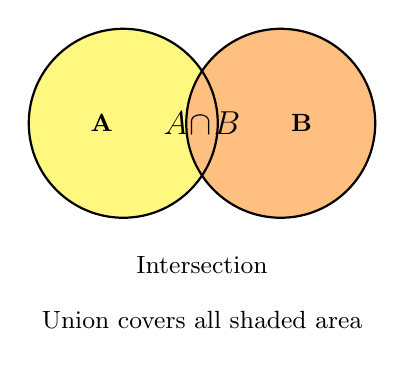
\begin{tikzpicture}[scale=1, every node/.style={font=\small}]
  % Circles for A and B
  \fill[yellow!50]   (-1,0) circle (1.2);
  \fill[orange!50]    (1,0) circle (1.2);
  \draw[thick]      (-1,0) circle (1.2) node[left]  {\textbf{A}};
  \draw[thick]      ( 1,0) circle (1.2) node[right] {\textbf{B}};
  % Labels
  \node at (0,0) {\large \(A\!\cap\!B\)};
  \node at (0,-1.8) {\small Intersection};
  \node at (0,-2.5) {\small Union covers all shaded area};
\end{tikzpicture}
\end{center}
\end{frame}

% ------------------------------------------------------------------------
\begin{frame}{Summary of Similarities}
\begin{itemize}
  \item \textbf{Cosine / Adjusted Cosine:} angle–based, handles centering.
  \item \textbf{Pearson:} mean–centered per item, good for item–based CF.
  \item \textbf{Spearman:} rank–based, robust to non-linear scales.
  \item \textbf{MSD:} direct squared difference, easy intuition.
  \item \textbf{Jaccard:} set overlap, suited to implicit/binary data.
\end{itemize}
\begin{center}
  \emph{Cosine remains a solid default choice for most applications.}
\end{center}
\end{frame}

% ------------------------------------------------------------------------
\begin{frame}[plain]
    \begin{center}
        {\LARGE \textbf{User-based Collaborative Filtering}}
    \end{center}
\end{frame}

% Overview slide
\begin{frame}{Overview}
\begin{itemize}
  \item Find users similar to the target user by comparing their ratings.
  \item Recommend items that those similar users liked, which the target user hasn't seen.
\end{itemize}
\end{frame}

% Example ratings slide
\begin{frame}{Example: Ratings Table}
\scriptsize
\begin{tabular}{l|ccccc}
                & Indiana Jones & Star Wars & Empire Strikes Back & Incredibles & Casablanca \\ \hline
\textbf{Bob}    & 4             & 5         & —                   & —           & —          \\
\textbf{Ted}    & —             & —         & —                   & —           & 1          \\
\textbf{Ann}    & —             & 5         & 5                   & 5           & —          \\
\end{tabular}
\end{frame}

% Similarity matrix slide
\begin{frame}{Step 1: Compute User–User Similarities}
\centering\scriptsize
\begin{tabular}{l|ccc}
       & \textbf{Bob} & \textbf{Ted} & \textbf{Ann} \\ \hline
\textbf{Bob} & 1.0          & 0.0          & 1.0          \\
\textbf{Ted} & 0.0          & 1.0          & 0.0          \\
\textbf{Ann} & 1.0          & 0.0          & 1.0          \\
\end{tabular}

\vspace{1em}
\emph{Bob’s top neighbors: Ann (1.0), Ted (0.0)}
\end{frame}

% Candidate generation slide
\begin{frame}{Step 2: Generate Candidates}
\begin{enumerate}
  \item Take Bob’s top neighbor(s): Ann (similarity = 1.0).
  \item Collect items Ann rated that Bob hasn’t:
    \begin{itemize}
      \item \textit{Empire Strikes Back}, \textit{Incredibles}
    \end{itemize}
\end{enumerate}
\end{frame}

% Scoring slide
\begin{frame}{Step 3: Score Candidates}
\normalsize
Normalize ratings to $[0,1]$ (e.g.\ 5 stars $\mapsto1.0$), then weight by similarity:
\[
\text{score}(i)
= \sum_{u\in\{\text{Ann}\}}
  \bigl(\mathrm{sim}(u,\text{Bob})\times\mathrm{normRating}(u,i)\bigr).
\]
Here Ann’s ratings $\to1.0$ and $\mathrm{sim}(\mathrm{Ann},\mathrm{Bob})=1.0$, so
\[
\text{score}(\textit{Empire}) = 1.0\times1.0 = 1.0,\quad
\text{score}(\textit{Incredibles}) = 1.0.
\]
\end{frame}

% Filtering & recommendation slide
\begin{frame}{Step 4: Filter \& Recommend}
\begin{itemize}
  \item Remove items Bob has already rated (none of these).
  \item Both candidates tie at score 1.0; choose \textit{Empire Strikes Back} as a recommendation.
\end{itemize}
\end{frame}

% Pipeline summary slide
\begin{frame}{User‐Based CF Pipeline}
\begin{enumerate}
  \item \textbf{Build rating matrix:} users $\times$ items.
  \item \textbf{Compute similarity matrix:} user–user (e.g.\ cosine).
  \item \textbf{Neighbor lookup:} top-$K$ similar users for target.
  \item \textbf{Candidate gen.:} items neighbors rated \(\setminus\) items target rated.
  \item \textbf{Score candidates:} weighted by similarity \& neighbor ratings.
  \item \textbf{Filter \& select:} exclude seen; sort by score; present Top-$N$.
\end{enumerate}
\end{frame}

% ------------------------------------------------------------------------
\begin{frame}[plain]
    \begin{center}
        {\LARGE \textbf{Item-based Collaborative Filtering}}
    \end{center}
\end{frame}

% Overview slide
\begin{frame}{Why Item‐Based CF?}
\begin{itemize}
  \item Items are \emph{stable} (a book remains a book), users' tastes may drift.
  \item Catalog size \(\ll\) user base \(\implies\) smaller similarity matrix.
  \item New‐user friendliness: as soon as a user interacts with one item, you can recommend similar items.
\end{itemize}
\end{frame}

% Ratings table
\begin{frame}{Example: Ratings Matrix}
\scriptsize
\begin{tabular}{l|ccc}
                & \textbf{Bob} & \textbf{Ted} & \textbf{Ann} \\ \hline
\underline{Indiana Jones}         & 4 &  &  \\
\underline{Star Wars}             & 5 &  & 5 \\
\underline{Empire Strikes Back}   &  &  & 5 \\
\underline{Incredibles}           &  &  & 5 \\
\underline{Casablanca}            &  & 1 &  \\
\end{tabular}
\end{frame}

% Cosine formula
\begin{frame}{Cosine Similarity Between Items}
\[
\mathrm{sim}(i,j)
= \frac{\sum_{u\in U_{ij}} r_{u,i}\,r_{u,j}}
       {\sqrt{\sum_{u\in U_{ij}} r_{u,i}^2}\;\sqrt{\sum_{u\in U_{ij}} r_{u,j}^2}}
\]
\begin{itemize}
  \item \(U_{ij}\): users who rated both items \(i\) and \(j\).
  \item Here, ratings are non‐zero only in our tiny example, so many similarities collapse to 0 or 1.
\end{itemize}
\end{frame}

% Similarity matrix
\begin{frame}{Step 1: Compute Item–Item Similarities}
\scriptsize
\centering
\begin{tabular}{l|ccccc}
               & \textbf{Indiana} & \textbf{Star Wars} & \textbf{Empire SB} & \textbf{Incredibles} & \textbf{Casablanca} \\ \hline
\textbf{Indiana Jones}       & 1 & 1 & 0 & 0 & 0 \\
\textbf{Star Wars}           & 1 & 1 & 1 & 1 & 0 \\
\textbf{Empire Strikes Back} & 0 & 1 & 1 & 1 & 0 \\
\textbf{Incredibles}         & 0 & 1 & 1 & 1 & 0 \\
\textbf{Casablanca}          & 0 & 0 & 0 & 0 & 1 \\
\end{tabular}
\end{frame}

% Recommendation for Bob
\begin{frame}{Step 2: Recommend for Bob}
\begin{enumerate}
  \item Bob’s known likes: \textit{Star Wars}.
  \item Look up all items similar to \textit{Star Wars}:
    \[
      \{\,\underline{\text{Indiana Jones}},\,
              \underline{\text{Empire SB}},\,
              \underline{\text{Incredibles}}\}
    \]
  \item Score each by its similarity to \textit{Star Wars} \(\times\) Bob’s rating of \textit{Star Wars} (5).
  \item Since \(\mathrm{sim}=1\) for all three and Bob’s rating=5,
    \[
      \text{score} = 1\times5 = 5.
    \]
  \item Filter out items Bob already rated (none of these).
  \item Final recommendations (tie): \textit{Indiana Jones}, \textit{Empire Strikes Back}, \textit{Incredibles}.
\end{enumerate}
\end{frame}

% Pipeline summary
\begin{frame}{Item‐Based CF Pipeline}
\begin{enumerate}
  \item \textbf{Build ratings matrix:} items \(\times\) users.
  \item \textbf{Compute similarity matrix:} item–item (e.g.\ cosine).
  \item \textbf{For target user:}
    \begin{itemize}
      \item Gather items they’ve rated.
      \item For each, fetch its top‐\(K\) similar items.
      \item Aggregate \& score candidates by \(\sum r_{u,i}\,\mathrm{sim}(i,\cdot)\).
      \item Remove already‐seen items.
      \item Present Top‐\(N\).
    \end{itemize}
\end{enumerate}
\end{frame}

% ------------------------------------------------------------------------
% \begin{frame}[plain]
%     \begin{center}
%         {\LARGE \textbf{Item-based Collaborative Filtering}}
%     \end{center}
% \end{frame}


\end{document}